\documentclass[letterpaper]{article}

\usepackage{natbib,alifeconf}  %% The order is important
\usepackage{amsmath}
\usepackage{amsfonts}
\usepackage{graphicx}
\usepackage{subcaption}
\usepackage{xspace}
\usepackage{needspace}
\usepackage{pbox}
\usepackage{hyperref}

\newcommand{\gv}{$g$-vector}
\newcommand{\phv}{$\phi$-vector}
\newcommand{\invv}{\ensuremath{\rotatebox[origin=c]{180}{\textrm{v}}}\xspace}

\title{Acclivation of Virtual Fitness Landscapes}
\author{Ben Kovitz$^{1}$, Dave Bender$^{1}$, \and Marcela Poffald \\
\mbox{}\\
$^1$Fluid Analogies Research Group, Indiana University, Bloomington, IN 47408 \\
bkovitz@indiana.edu}

\begin{document}
\maketitle

\begin{abstract}
Simple spreading-activation networks are shown to exhibit acclivation of a
``virtual fitness landscape''. That is, the fitness function faced by part of
the genome, when the remainder of the genome is held constant, becomes
progressively more smoothly sloped, or hill-shaped.

Applied directly to the phenotype, the original fitness function is filled
with traps and local optima. The topology of the spreading-activation network
experiences indirect selective pressure to make the fitness landscape become
less rugged as seen by a numerical vector that is fed into the network.
The evolving topology exploits regularities in the original fitness
function, such as a ``ridge'' and regularly spaced ``bumps'', to make it
easier for the vector to navigate the fitness landscape by simple
hill-climbing.

This shows that under appropriate conditions, complex \mbox{epistasis} and
non-locality of genotype--phenotype mapping can improve evolvability. These
conditions are typical of those found in nature, where behavior and phenotypes
are produced mainly by cascades of activity through a graph and coordination
among the parts of the phenotype is a precondition of successful survival and
reproduction.

\end{abstract}

% Relevant topics to search in the literature:
%
% how much epistasis is there in natural genomes?
% crosstalk in metabolic networks

\section{Virtual Fitness Functions}
@@.\footnote{\cite{hogeweg2012toward}.}

Any part of a genome is selected against a \textit{virtual fitness function}
resulting from the rest of the genome and the fitness function faced by the
genome as a whole. If the whole-genome fitness function reflects the influence
of the environment on the genome, then the virtual fitness function represents
the same for a part of the genome, whose environment includes the rest of
the genome.

Let a set of genotypes $G$ have a mapping $m_{G} : G \rightarrow \Phi$ to a set
of phenotypes $\Phi$, and let $w_\Phi : \Phi \rightarrow \mathbb{R}$ be the
fitness function for the phenotypes. Then $w_G : G \rightarrow \mathbb{R}$, the
fitness function for the whole genome, is the composition of these functions,
$w_G(g) = w_\Phi(m_{G}(g))$.

If we divide the genome into two parts $G_1$ and $G_2$, then each genotype $g
\in G$ consists of a $g_1 \in G_1$ and a $g_2 \in G_2$, in which each $g_2$
defines a partial-genotype--phenotype mapping $m_{g_2} : G_1 \rightarrow
\Phi$. That is, if we hold part of the genome constant, say by fixing $g_2$,
this defines a mapping from all possible values of the rest of the genome,
$g_1$, to corresponding phenotypes. If we reverse $g_1$ and $g_2$, then of
course we get the opposite partial-genotype--phenotype mapping, $m_{g_1} : G_2
\rightarrow \Phi$.

These mappings, in turn, define virtual fitness functions $v_{g_2}(g_1) =
w_\Phi(m_{g_2}(g_1))$ and $v_{g_1}(g_2) = w_\Phi(m_{g_1}(g_2))$. As mutations
and crossovers can alter either or both of $g_1$ and $g_2$, the partial
genomes $G_1$ and $G_2$ coevolve cooperatively, each selected by
the fitness functions $v_{g_1}$ and $v_{g_2}$, which vary among all the
individuals and vary each generation.

Let \textit{evolvability} be defined in some reasonable way (there are many),
so that greater evolvability implies some advantage in navigating a fitness
landscape upward faster or further over succeeding generations. Let $g_a,g_b
\in G$ be two individuals in the same population and the same generation.
Assuming no other advantages favoring either $g_{a1}$ or $g_{b1}$, if $g_{a1}$
presents its mate $g_{a2}$ with a virtual fitness function $v_{g_{a1}}$ that
$g_{a2}$ finds more evolvable than $v_{g_{b1}}$ is for $g_{b2}$, then the
descendants of $g_a$ will evolve faster or further than the descendants of
$g_b$ (according to how evolvability is defined).

Therefore each partial genome is under selective pressure to create a virtual
fitness landscape for the other partial genome that gives the latter greater
evolvability. To illustrate with an unrealistically simple example, if the eye
and the arm are governed by separate sets of genes, and some arm shapes make
it easier for the eye to evolve, then there is selective pressure favoring
alleles for those arm shapes. All other factors being equal, evolution favors
arms that make eyes easier to evolve. This selective pressure happens
indirectly; in any single generation, greater fitness wins. But over successive
generations, descendants of organisms with greater evolvability will tend to
have greater fitness than organisms with lesser evolvability.@@cite-Altenberg?

The above considerations make no difference for homogeneous genomes, where
every part of each genotype undergoes mutation and crossover the same as every
other part and exerts the same effect on the phenotype or on the total fitness
as every other part. However, if $G_1$ and $G_2$ vary according to different
operators and/or affect the phenotype or total fitness differently, there is
potential for each part to seek values that make the other part more
evolvable, resulting in a period of progressively increasing evolvability for
the organism as a whole.

In the rest of this paper, we examine a natural and common way for this
synergy to occur: when $g_1$ consists of a vector of real numbers (``knobs'')
and $g_2$ consists of a network that provides connections through which the
numbers from $g_1$ interact.

\section{Acclivation}

As is well known, a genome consisting of a vector of numbers, where mutations
alter the numbers by small amounts, evolves most easily against a hill-shaped
fitness function. In a hill-shaped fitness function, local increases in
fitness correlate perfectly with movement toward the peak of the whole fitness
landscape. The more ``rugged'' the landscape, the weaker is this correlation,
so that following the local gradient can lead organisms to become stuck at
local maxima, which might be very low, and from which they cannot escape by
local mutations (though they might escape by crossover).@@cite-Kauffman

Therefore, if a vector of numbers faces a rugged fitness landscape, with
difficult features such as low local peaks and impassable moats, we can
improve its evolvability for a vector of numbers by making its fitness
function more hill-shaped. Let us call the process of making a fitness
landscape more hill-shaped \textit{acclivation.}

So, in a genome where $G_1$ is a vector of numbers that mutate by small
amounts, and $G_2$ is a directed graph that feeds the numbers in $G_1$ through
nodes that perform some function on the numbers from their input edges,
eventually leading to a phenotype whose fitness determines the fate of the
whole organism, we should expect selective pressure for genotypes $g_2 \in
G_2$ to produce mappings that induce acclivation on the virtual fitness
functions $v_{g_2}$. Evolution should favor graphs that put knobs in a
position where they can hill-climb successfully.

\section{Genome for Experimentation}

To test the preceding hypothesis in a form in which acclivation will be
visually apparent on plots printed on paper, we limit ourselves to genomes
where $g_1$ and the phenotype are 2-dimensional vectors and $g_2$ is a graph
connecting them.  The whole genome is a directed graph where:
\begin{enumerate}
   \item Two nodes, called the \textit{knobs}, $k_1$ and $k_2$, are designated
      to each hold a number in $[-1.0, +1.0]$, called an \textit{initial
      activation}.
   \item Two other nodes, $p_1$ and $p_2$, are designated to hold the
      phenotype.
   \item Each edge has a weight of either $+1.0$ or $-1.0$.
\end{enumerate}

\subsection{Genotype--Phenotype Mapping}

The phenotype is determined by a process of spreading activation, run for
10 timesteps. Each timestep, the initial activations from the knobs flow into
adjacent nodes, producing a number in $[-1.0, +1.0]$ called the node's
\textit{activation}. The activation of a node $a_j$ at timestep $t+1$ is
calculated according to the following function:
\[
   a_j(t+1) = T(a_j(t) + \sum_iW_{ij}a_i(t))
\]
where $W_{ij}$ is the weight of the incoming edge, if any, from node $i$ to
node $j$, and $T$ is the following transfer function:
\[
   T(x) = \frac{2}{1+\exp(-Sx)}-1
\]
where $S=2.1972274554893376$. This constant gives $T$, when iterated,
attractors at $\pm0.5$ and a repellor at 0.

If a node does not have an activation at time~$t$, then it does not figure
into the above sum for calculating any other node's activation. At time~$t=0$,
only the knobs have activations.

The phenotype is the vector $(a_{p_1}(10), a_{p_2}(10))$, i.e.~the activations
of the phenotype nodes after 10 timesteps. If $p_1$ or $p_2$ has not received
an activation after 10 timesteps, then the genotype has no phenotype and is
given a fitness of~0.0. This can happen if no edges provide a path from a knob
to $p_1$ or~$p_2$.

\subsection{Mutation and Crossover}

In generation 0 of the first epoch in each experiment, the population consists
of genotypes containing only the two knob nodes and the two phenotype nodes,
with up to four randomly placed edges with weights randomly chosen from $\{-1,
+1\}$, and the knobs' initial activations chosen uniformly from $[-1.0, 1.0]$.

Each organism of each successive generation is generated by the following
algorithm:
\begin{enumerate}
  \item Randomly choose mutation or crossover. Crossover has a low probability,
    usually $0.02$ or $0.05$.
  \item If mutation was chosen, choose a parent organism by tournament selection
    from the previous population, and perform one of these mutations, chosen at
    random: add a node, remove a node, add an edge, remove an edge, move an
    edge, or turn a knob. Knob-turning has a probability roughly equal to the
    sum of all the graph-edit mutations. Depending on the experiment, turning a
    knob chooses a knob delta from ${-0.02, +0.02}$ or from a normal
    distribution with mean 0 and $\sigma = 0.0$.
  \item If crossover was chosen, choose two parent organisms by tournament
    selection from the previous population, choose subsets of nodes from each,
    and randomly allow nodes to carry through to the child organism.
\end{enumerate}
Population sizes range from 80 to 800 depending on the experiment. We omit some
details of the variation operator here for lack of importance. The source code
is publicly available at
\href{https://github.com/bkovitz/sa}{https://github.com/bkovitz/sa}.

\section{Experiments}

In each experiment, we run the genome defined above, perhaps with a slight
variation, against a different family of fitness functions, and see what
virtual fitness functions emerge. We only plot $v_{g_2}$, the virtual
fitness function seen by the knobs, since we know of no way to plot fitness
functions seen by a graph.

Each experiment tries a ``family'' of fitness functions, because each
experiment's fitness function has a constant that changes randomly once per
epoch: every 20 generations. This constant moves the peak of the fitness
function to different places in phenotype space.

Frequently moving the peak is necessary to induce strong selective pressure
favoring evolvability rather than organisms that only approximate the current
peak.@@cite Each new epoch is thus a race to approach the new peak. The most
evolvable genotypes' lineages will approach the new peak faster than their
less evolvable competitors. In this way, the experiments tend to reward
evolvability especially strongly.

\subsection{Experiment 1: Narrow Ridge}

\begin{figure*}[t]
   \centering
   \begin{subfigure}[b]{0.2\textwidth}
   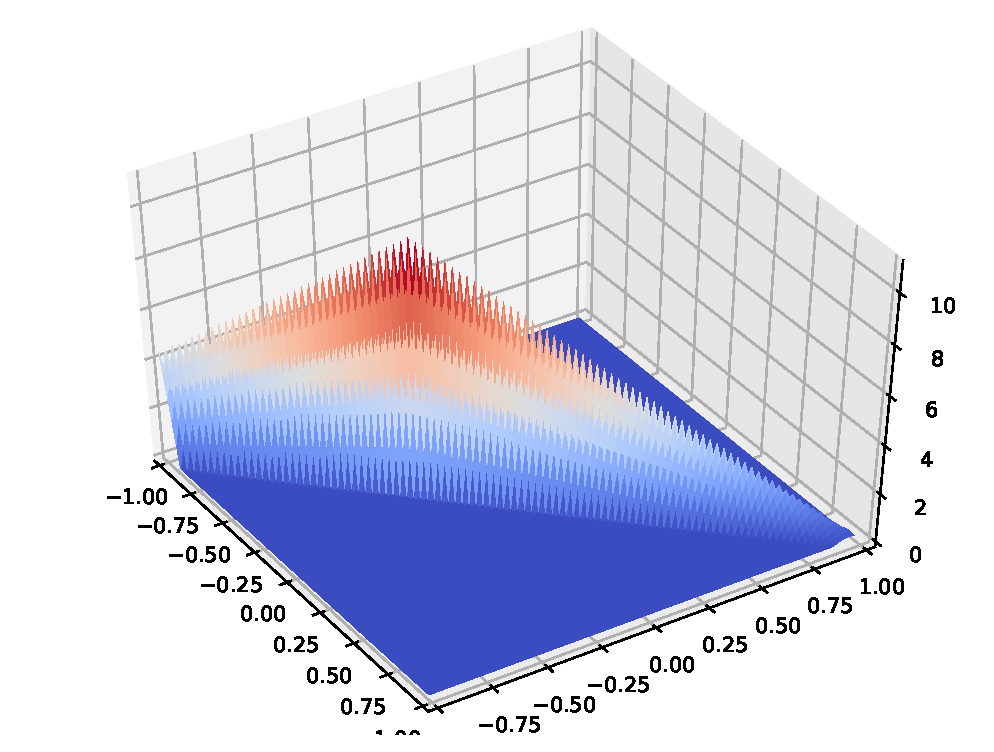
\includegraphics[width=2in]{yxline2-phfunc.eps}
   \caption{Phenotype fitness}
   \label{yxline2-phfunc}
   \end{subfigure}
   \begin{subfigure}[b]{0.2\textwidth}
   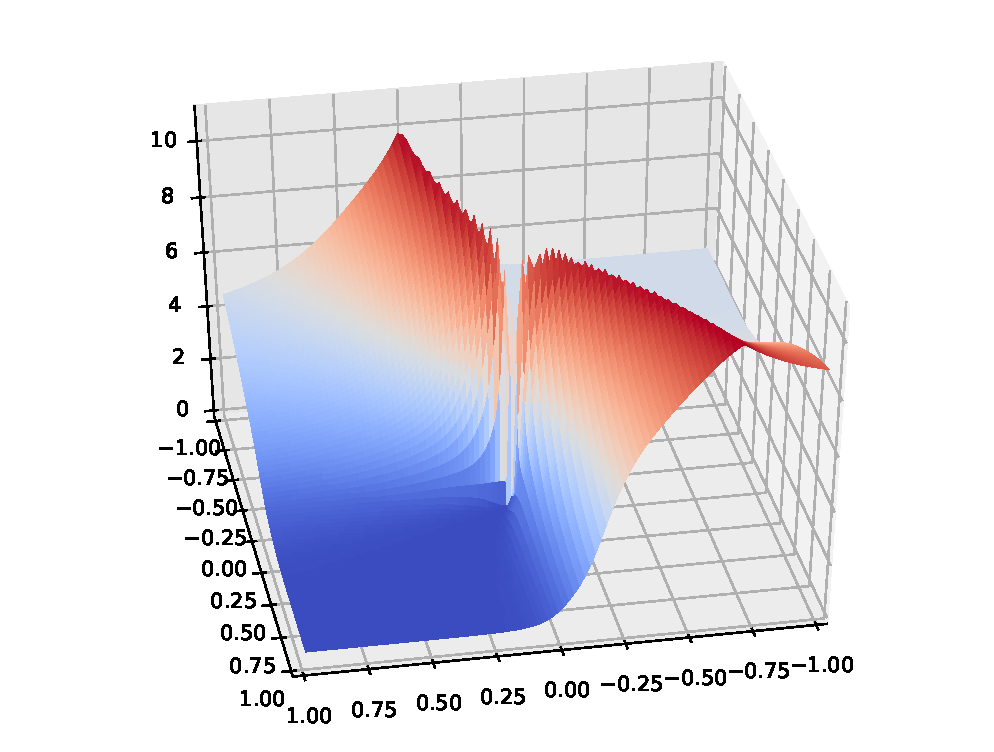
\includegraphics[width=2in]{yxline2-vfunc.eps}
   \caption{Virtual fitness}
   \label{yxline2-vfunc}
   \end{subfigure}
   \begin{subfigure}[b]{0.2\textwidth}
   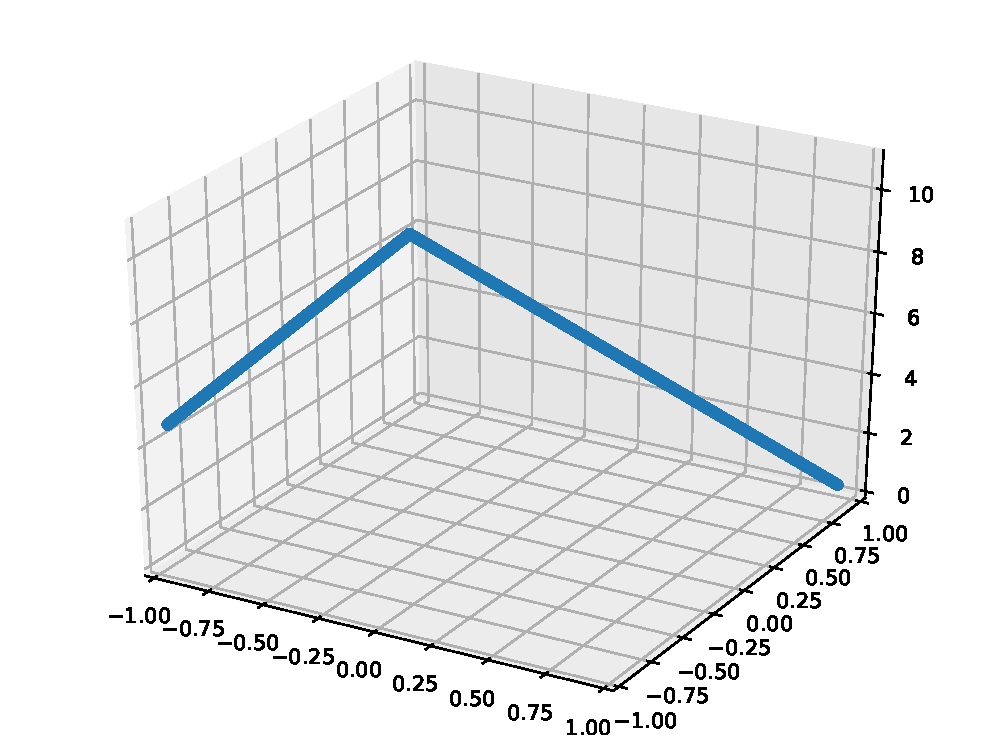
\includegraphics[width=2in]{yxline2-phrange.eps}
   \caption{Phenotype range}
   \label{yxline2-phrange}
   \end{subfigure}
   \begin{subfigure}[b]{0.2\textwidth}
   \includegraphics[width=2in]{yxline2.pdf}
   \caption{Genotype}
   \label{yxline2-genotype}
   \end{subfigure}

   \begin{subfigure}[b]{0.2\textwidth}
   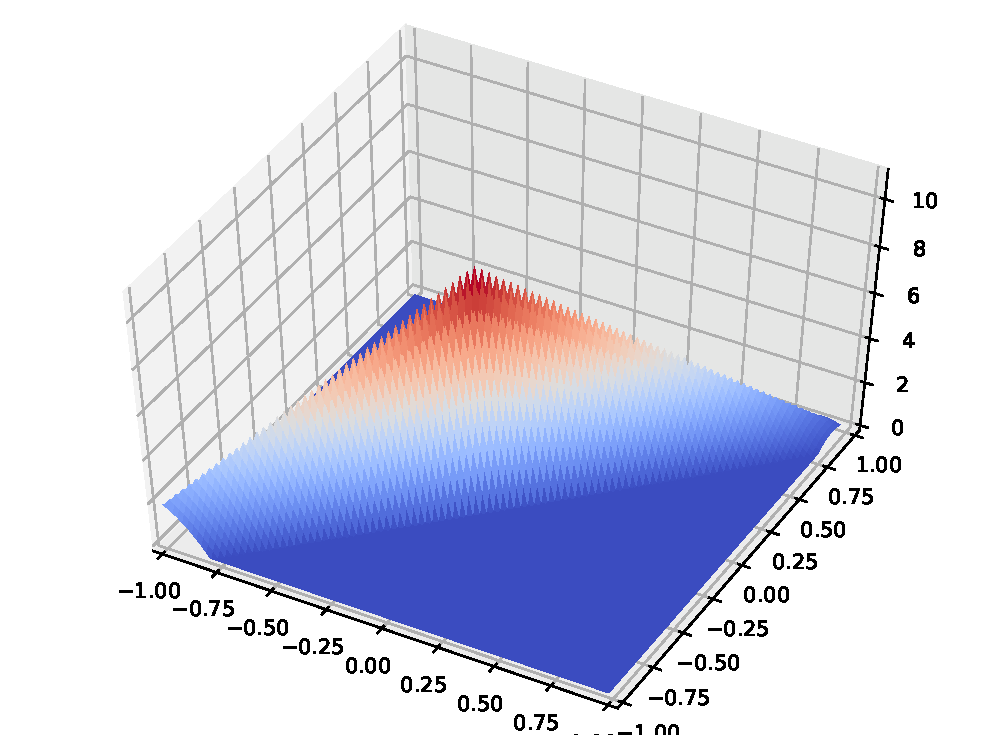
\includegraphics[width=2in]{yxline1-phfunc.eps}
   \caption{Phenotype fitness}
   \label{yxline1-phfunc}
   \end{subfigure}
   \begin{subfigure}[b]{0.2\textwidth}
   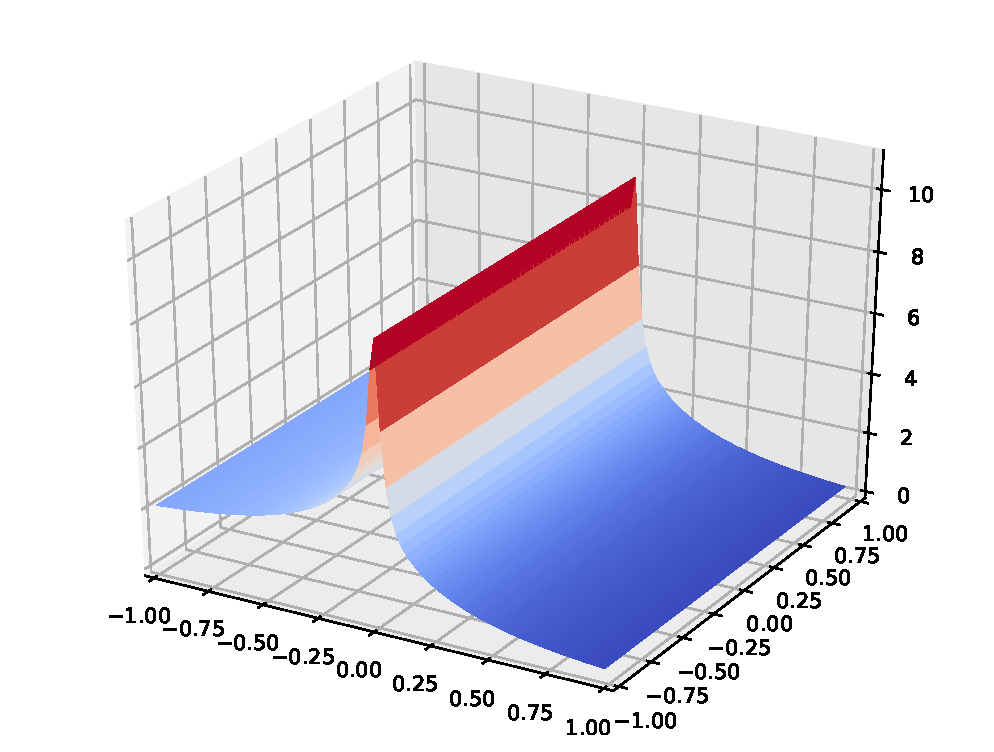
\includegraphics[width=2in]{yxline1-vfunc.eps}
   \caption{Virtual fitness}
   \label{yxline1-vfunc}
   \end{subfigure}
   \begin{subfigure}[b]{0.2\textwidth}
   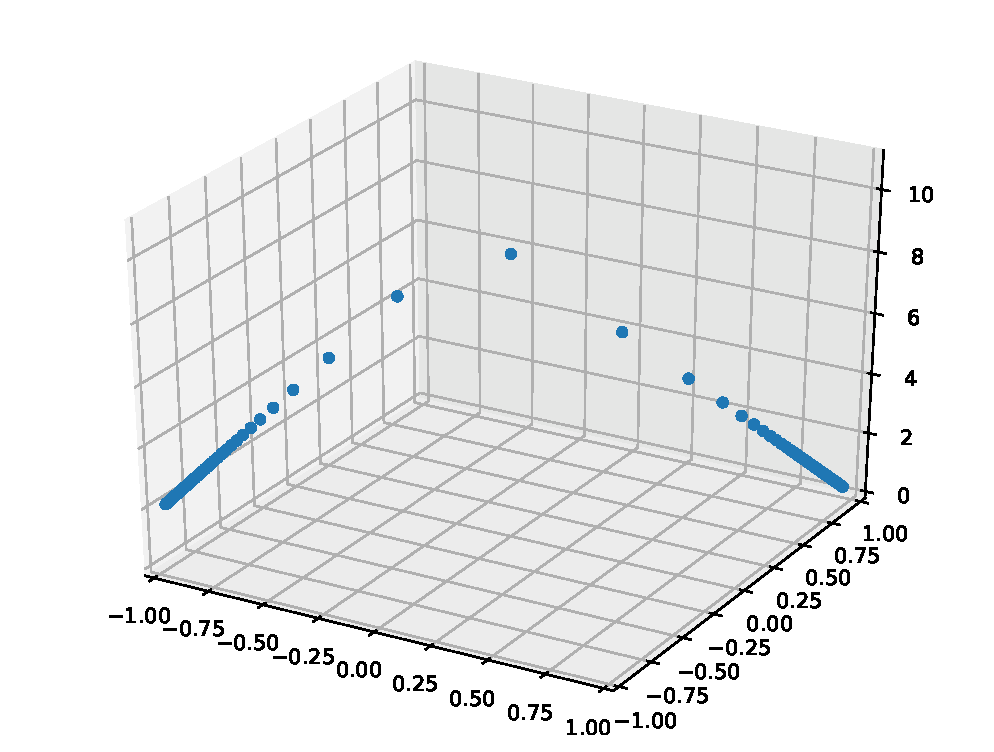
\includegraphics[width=2in]{yxline1-phrange.eps}
   \caption{Phenotype range}
   \label{yxline1-phrange}
   \end{subfigure}
   \begin{subfigure}[b]{0.2\textwidth}
   \includegraphics[width=2in]{yxline1.pdf}
   \caption{Genotype}
   \label{yxline1-genotype}
   \end{subfigure}


   \caption{Experiment~1: Narrow Ridge. (\subref{yxline2-phfunc}) has a
   ridge radius $R$ of $0.1$; (\subref{yxline1-phfunc}) has a ridge radius
   of $0.2$. $x,y$ values in phenotype ranges indicate points in phenotype
   space that have a preimage in knob space when the knobs are mapped through
   $m_{g_2}$. The $z$ values are the fitnesses of those phenotypes (the same
   as in (a) and (e)). Knobs are shown at the top of each graph, phenotype
nodes at the bottom. Numbers in nodes are activation levels at the end of
spreading activation. Numbers preceded by ``i='' are initial activation
levels.}
   \label{fig:narrow-ridge}
\end{figure*}

In this experiment, we run the experimental genome against this fitness
function, plotted in Figures~\ref{yxline2-phfunc} and~\ref{yxline1-phfunc}:
\[
   w_\Phi(\phi) = 10.0 \cdot \hat{d}(\phi, P) \cdot \invv(|p_2 - p_1|; R)
\]
where
$R$ is a small radius, set to $0.1$ or $0.2$ in different runs of the
experiment,
$P$ is a point (the peak) chosen randomly along the $y=x$ line each epoch,
$\hat{d}(\phi, P)$ is a measure of the proximity of $\phi$ to $P$ equal to
$0.0$ for the maximum possible distance $M$ and $1.0$ for zero distance:
\[
  \hat{d}(\phi, P) = \frac{\max - d(\phi, P)}{\max}
\]
and \invv is the ``inverted-v function'' (like an inverted-U function but
peaking sharply at $x=0$ and returning zero outside the radius $R$):
\[
   \invv(x; R) =
   \begin{cases}
      0 & \text{if } |x|>R \\
      1 - (\frac{x}{R})^2 &
      \text{if } |x|\leq R
   \end{cases}
\]
So, the phenotype is rewarded up to 10.0 points for proximity to $P$, but only
if the phenotype lies along a narrow ridge running diagonally across phenotype
space. The diagonal direction is chosen to frustrate direct evolution: if the
knobs–-phenotype mapping is simply the identity function, $m_{g_2}(g_1)=g_1$,
then even if the phenotype lies along the ridge, a single knob-turn mutation
is likely to throw it off the ridge.

In Figure~\ref{fig:narrow-ridge} we see two genotypes that evolved in this
experiment, illustrating two ways that the graph $g_2$ can provide a virtual
fitness function that affords more evolvability for the knobs than the
phenotype fitness function does.

First, the virtual fitness function in (\subref{yxline2-vfunc}) illustrates
acclivation: is much wider and more gently sloped than the original fitness
function. The image of the ridge in knob-space is much easier to find and
navigate than the ridge in phenotype-space.

Second, both virtual fitness functions, but especially the one in
(\subref{yxline1-vfunc}), illustrate another way to gain evolvability:
simply exclude the bad parts of the phenotype space from the range of
$m_{g_2}$. The phenotype ranges plotted in (\subref{yxline2-phrange})
and (\subref{yxline2-phrange})
do not permit \text{any} knob setting to map anywhere but along the very
center of the ridge. The vast ocean of zero-fitness points that lie off the
ridge in phenotype space is unreachable. The graphs accomplish this by simply
disconnecting one of the knobs.

The relative sparsity of dots plotted in the middle of the phenotype range
in (\subref{yxline1-vfunc}) indicates that small knob-turnings in that range
move quickly, or relatively long distances, through phenotype space. The
relative density at the extremes indicates that knob-turnings move slowly
through phenotype space there. Note that this is the opposite of what would
promote greater evolvability for the knobs, since a knob-turning mutation is
likely to overshoot the peak or lose a lot of fitness when the phenotype is
near the peak, and will have little effect on the phenotype when the phenotype
is far from the peak.

\subsection{Experiment 2: Razorback}

In this experiment, we run the experimental genome against this fitness
function, plotted in Figure~@@:
\[
   w_\Phi(\phi) = 10.0 \cdot \hat{d}(\phi, P)
                       \cdot \invv(|p_2 - p_1|; R)
                       + \text{waves}(\phi; 30)
\]
where:
\begin{itemize}
  \item[ ]
    $P$ is a point (the peak) chosen randomly along the $y=x$ line each epoch;

  \item[ ]
$\hat{d}(\phi, P)$ is a measure of the proximity of $\phi$ to $P$ equal to
$0.0$ for the maximum possible distance and $1.0$ for zero distance:
\[
  \hat{d}(\phi, P) = \frac{\max - d(\phi, P)}{\max}
\]

  \item[ ]
    \invv is the ``inverted-v'' function: like an inverted-U function but
    peaking sharply at $x=0$ and returning zero outside the radius $R$, set to
    0.1 or 0.2 on different runs of the experiment:
\[
   \invv(x; R) =
   \begin{cases}
      0 & \text{if } |x|>R \\
      1 - (\frac{x}{R})^2 &
      \text{if } |x|\leq R
   \end{cases}
\]

  \item[ ]
    and ``waves'' is a function that adds regular undulations, giving the
    overall fitness function an ``egg carton'' look:
\[
  \text{waves}(\phi; \nu) = \cos(\nu p_1)
                            \cdot
                            \sin(\nu (p_2 + \frac{\nu}{2})
\]
\end{itemize}

So, this function rewards the phenotype up to 10 points for proximity to
$P$, but only if the phenotype lies along a narrow ridge running diagonally
across phenotype space, complicated by the addition of a regular pattern of
undulations. The undulations add local minima throughout the fitness
landscape to trap searches that merely follow the local gradient.

\subsection{Experiment 3: Circle}

In this experiment, we run the experimental genome against this fitness
function:
\[
  w_\Phi(\phi) = 10.0 \cdot \hat{d}(\phi, P)
                      \cdot \invv((p_1^2 + p_2^2) - r^2; R)
\]
where $r$ is the radius of a circle, $R$ is the ridge radius as in the first
experiment, and $P$ is a point (the peak) chosen randomly along the circle
at the start of each epoch. In words, the phenotype is rewarded up to 10.0
points for proximity to the peak, but only if the phenotype lies within $R$
of the perimeter of the circle---a circular ridge. We set $r=0.5$ and $R=0.2$.

\subsection{Experiment 4: Moats}

\section{Observations and Discussion}

The main result is that when a genome can evolve its genotype--phenotype
mapping and consists of continuously varying ``knobs'' as well as a
discontinuously varying topology or ``graph'', the graph is under selective
pressure to present the knobs with a virtual fitness function that is easy for
the knobs to follow upward---a hill-shaped function. This can't make any
rugged fitness landscape smooth and tractable, of course, but it can reduce
ruggedness in many situations.

The selective pressure for acclivation is strongest if fitness is set up in a
way that especially rewards evolvability, such as a fitness function with a
constant that changes occasionally, shifting the peak. The family of
genotype--phenotype mappings that the set of possible graphs can implement must
itself afford an evolutionary path along which it can ``acclivate'' the virtual
fitness function in response to success and failure of knob-turning.

Properly speaking, the graph evolves a knob--phenotype mapping, not a
genotype--phenotype mapping, since the graph is itself part of the genotype.
But we will use the latter term since it's more standard and the
knob--phenotype mappings studied here relate most closely to what are called
genotype--phenotype mappings elsewhere in the literature.

\subsection{Genetic Memory}

Over many generations, the graph accumulates a ``memory'' of the family of
whole-genome fitness functions, encoded in the form of \textit{bias} in the way
its lineage searches the phenotype space. This bias reflects invariants in the
fitness family, such as where ridges occur and how they're oriented, moat size,
and where zero-fitness ``deserts'' consistently lie.

The knobs exploit this bias by wandering only in regions with high fitness or
regions where following (virtual) gradients tends to lead reliably to
improvements. The graph also exploits the biased search that it has evolved,
through discontinuous leaps rather than incrementally (but see ``Virtual
Knobs'' below).

Knobs themselves cannot accumulate useful bias beyond being positioned where
they will be mapped to high-quality phenotypes. This bias can be effective,
though: in a single population, there may be several lineages with knobs
positioned far apart, each ready to capitalize if the whole-genome fitness
function or the genotype--phenotype mapping changes to favor them again.

In our experiments, we frequently witnessed the decay of a population's genetic
memory. Many times, a population that was responding quickly to shifts of the
fitness peak, moving rapidly toward it one knob-turn per generation, lost its
ability to do this when a few epochs went by with little or no movement in the
fitness peak. When the peak stayed constant too long, selective pressure
favored canalization: genotype--phenotype mappings that held the phenotype at
the peak in the face of most mutations. In that circumstance, if knob-turning
alters the phenotype at all, it lowers fitness, so selective pressure favors
rendering it inert---that is, making a genotype--phenotype mapping in which all
points in knob-space map to the same point in phenotype space.

Genetic memory also frequently decayed when a knob had a value of $-1.0$,
$0.0$, or $+1.0$. At the extremes, a knob-turning mutation that goes beyond the
limit has no effect. So, at these times, knob-turning often lost its
sensitivity to the virtual fitness gradient---and so improvements in fitness
had to come by graph-edits alone, which can spoil previous acclivation. When a
knob is 0.0, a knob-turning mutation has much smaller effect than at other
values, mostly due to a peculiarity of the transfer function (see below).
Consequently, knob-turning lost its sensitivity to the virtual fitness
gradient, so selective pressure again favored radical graph edits that spoil
acclivation.

\subsection{No Measure of Acclivation}

We present no measure how often acclivation occurs or how much. We tried
measuring the ``acclivity'' of a virtual fitness function by running a
hill-climbing algorithm on it, but this yielded ambiguous results. Does a
higher fitness reached by the hill-climber mean higher acclivation? Not the
genotype--phenotype mapping is constrained to a small range centered on the
peak. Then the hill-climber reaches high fitness even though the virtual
fitness function is not very hill-shaped. Do we measure how far the average
hill-climber climbs?  That measure also gives misleading results for many
virtual fitness functions. How should neutral plateaus count into the acclivity
measure? How much should parts of the landscape far from the current knob
settings count?

So, in this paper we limit ourselves to interesting qualitative observations
of the virtual fitness functions that emerged and analysis of their
significance.

\subsection{Nonlocality and Epistasis}

@@

\subsection{Mutation Rate}

Allowing one mutation per generation is somewhat unrealistic biologically,
since in living organisms, longer genomes have more opportunity to mutate;
nature does not limit mutations to one per organism per generation. When we
allowed a number of mutations proportional to the size of a genotype, the
genotypes tended to ``bloat'', acquiring hundreds of disconnected nodes and
edges. The problem is that when larger genotypes can make more mutations per
generation, they have no incentive to optimize the way they respond to graph
mutations.  When each organism can only vary from its parent by a single
mutation, those who do not optimize their mutation exposure are at a
disadvantage in the race to the new peak at the start of each epoch. A lineage
with an unnecessarily large number of ways to make neutral mutations will tend
to lose those races to lineages with the minimal amount of ``padding''.

\subsection{Virtual Knobs}

We ran variations on the above experiments where nodes other than the knobs were
allowed to inherit constants. For example, we tried allowing non-knob nodes to
inherit an initial activation. Under this condition, successful organisms tended
to accumulate a collection of nodes with different constants, none of which were
connected to the knobs and only one of which was connected to a phenotype node.
They exploited the ``move edge'' mutation to make these collections of nodes
function as a virtual knob. Both knob nodes were often disconnected from the
rest of the graph.

The organisms seemed to prefer their virtual knobs. Virtual knobs are subject to
evolutionary pressure determining how fast they turn, i.e.~the probability
distribution of knob-turning deltas. The hard-coded knobs are limited to deltas
in the range of about $\pm0.02$. The evolved virtual knobs tended to turn much
faster than our hard-coded knobs.

When we removed nodes with constants, we tried allowing more than one edge
between nodes. The organisms evolved to exploit the ``add edge'' and ``remove
edge'' mutations as knobs. The number of edges between two nodes effectively
served as an adjustable multiplier.

To get the organisms to make use of our hard-coded knobs, necessary to examine
virtual fitness functions whose domain is the knob settings, we had to purge
the graph of all other constants capable of varying in small increments. This
severely reduces evolvability.

\begin{figure}[b]
  \centering
  \includegraphics[width=0.48\textwidth]{ratio.pdf}
  \caption{A graph from \citet{kovitz2015experiments} that evolved against a
    fitness function that rewards a constant ratio among the phenotype nodes,
  varying the absolute numbers once each epoch.}
  \label{fig:virtual-knob}
\end{figure}

\citet{kovitz2015experiments} reports experiments with ``cascading designs''
where graphs evolve genotype--phenotype mappings for greater evolvability, also
under pressure from fitness functions with constants that change once per epoch.
All nodes in those graphs inherit constants that can mutate a small amount in
each generation, like a knob. Those graphs, too, evolve virtual knobs, as shown
in Figure~\ref{fig:virtual-knob}. The node that links directly to all four phenotype nodes functions
as a virtual knob that approximately maintains an invariant relationship
among the phenotype nodes.

The other nodes, which occur in clusters, function as a large virtual knob for
making fine-tuning adjustments to individual phenotype nodes.  The relative
numbers of nodes in different clusters determine, in effect, the relative
frequency of ``virtual-knob mutations'' and graph edits that don't alter a
virtual knob. So, without a control for mutation frequencies explicitly provided
in the program, the organisms evolved their own.

There is no exact boundary around a virtual knob, since the same node can be
selected to implement continuous variation along some axis as well as implement
some part of graph topology (like maintaining an invariant relationship), or
switch between these roles in different mutations.

\subsection{The Transfer Function}

One might expect that nearly any transfer function typically used in simulated
activation networks would produce similar acclivation, but we found that a
simple $y=x$ function clamped within $[-1.0, 1.0]$, step functions, rectifier
functions, and letting the constant in the $T$ function stray too far from $S$
all produced much less acclivation as well as phenotypes of much lower fitness.
The graphs could not ``lock on'' to the ridge, making knob-turning nearly
useless for navigating up the fitness functions.

The $T$ function has a peculiar characteristic that makes it suitable for
these experiments, where the only constants in the genotype that are allowed to
vary in small increments are those in the knobs. $T$ is expansive in the range
$-.28 < x < .28$ and contractive everywhere else. When a constant input, as
from a knob, is fed into $T$ repeatedly ten times, this yields a function
$T(x+T(x+T(\ldots)))$, which is expansive in $-.14 < x < .14$ and contractive
everywhere else. This makes $T$ well suited to forming a wide variety of
functions that simultaneously dilate and compress different ranges of the
phenotype space, by composition with itself alone---without constants.
Activations from incoming edges $a_{i}$ beyond the first edge make a node
calculate the function $T(a + \sum_i a_i)$, giving compositions of $T$ the
ability to shift their output right or left.

Figure~@@ illustrates the compression of the phenotype space in the center of
knob space and the dilation toward the extremes. This virtual fitness function
evolved against a fitness function like that in experiment @@ but without the
``egg carton'': a simple diagonal ridge with no bumps. Note that the range of
expansion corresponds to compression of the phenotype function as seen through
$T$ and the range of contraction corresponds to dilation of the phenotype
function. (Where the image of a function contracts, the preimage dilates.)

Compositions of the linear transfer functions can shift phenotype space but they
can't dilate or compress it. This makes it harder, perhaps impossible, to
evolve an acclivated virtual fitness function. When the constant $S$ is varied
too far from that in $T$, the resulting function's range of expansion quickly
shrinks to a tiny region around $x=0$ or grows to nearly the whole interval
$[-1.0, 1.0]$.

The need to compose many instances of $T$ seems to be important. When we ran
simulations that iterated spreading activation 3 or 5 times instead of 10,
there was much less acclivation. 20 iterations seemed to have little effect.

\subsection{Biological Significance}

DNA, neurons, social specialization

expert perception?

@cite-chem-paper

\section{Conclusions}

\subsection{Limitations and Future Work}

@@how to quantify acclivity


\bibliographystyle{apalike}
\bibliography{acclivation} % replace by the name of your .bib file

\end{document}
